              
\documentclass[12pt]{article}
 \usepackage[margin=1in]{geometry} 
\usepackage{amsmath,amsthm,amssymb,amsfonts, graphicx, tikz, placeins}
\usetikzlibrary{positioning}
 
\newcommand{\N}{\mathbb{N}}
\newcommand{\Z}{\mathbb{Z}}
 
%\newenvironment{problem}[2][Problem]{\begin{trivlist}
%\item[\hskip \labelsep {\bfseries #1}\hskip \labelsep {\bfseries #2.}]}{\end{trivlist}}
%If you want to title your bold things something different just make another thing exactly like this but replace "problem" with the name of the thing you want, like theorem or lemma or whatever
 
\begin{document}
 
%\renewcommand{\qedsymbol}{\filledbox}
%Good resources for looking up how to do stuff:
%Binary operators: http://www.access2science.com/latex/Binary.html
%General help: http://en.wikibooks.org/wiki/LaTeX/Mathematics
%Or just google stuff
 
\title{Homework 1}
\author{Selma Wanna \\ SLW3429 \\ slwanna@utexas.edu} 
\maketitle
 
\section{Introduction}

Homework 1 focuses on investigating Principal Component Analysis (PCA) on MNIST data of handwritten digits. The goal is to learn about feature extraction and understand low-dimensional data projections through PCA. Once the training data set is mapped to a suitable lower dimensional representation, a K Nearest Neighbors classification method is implemented to correctly identify unknown test images.

\section{Methods}
Leveraging Principal Component Analsis (PCA), and its ability to project high dimensional data to lower dimensions while reducing the square projection error, is a critically important skill for a solid foundation in machine learning.
\bigbreak
\noindent
In order to use PCA, some preprocessing is required. First, mean normalization must occur, such that each image feature \(x\) in the training set of length \(M\) undergoes the following treatment.

\[\mu_{j} = \frac{1}{M}\sum_{i=1}^{M} {x}_{i}^{j} \]

\noindent
Thereafter, every \({x}_{i}^{j}\) must be replaced with \({x}_{j}-{\mu}_{j}\). This allows the mean of each feature to be 0. This is the end of the preprocessing steps required for the MNIST classification problem provided in homework 1. The steps which follow aim to  develop a projection of our training data to a lower dimensional space.
\bigbreak
\noindent
In order to leverage lower dimensionality, we must first determine the covariance of our training set data. To do so, we follow the equation below, where \(X\) represents the full image.

\[\Sigma = \frac{1}{M}\sum_{n=1}^{M}X_{n}X_{n}^{T}\]

\noindent
The calculation above is susceptible to incredibly high dimensionality given a large feature set. Luckily, \(\Sigma \) can be approximated by a matrix of lower rank, such that important feature variation is projected to a subspace whose dimensions are less than the dimensions of the original training set. In such cases, the following two step trick can be used to reduce the overall dimensionality of the matrix. Let \(\mu\) represent eigenvalues of the covariance matrix, and let \(\upsilon\) represent its eigenvectors. 

\[A^{T}A\upsilon = \mu\upsilon, A = [X_{1},X_{2},...X_{M}] \]

\[A A^{T}A\upsilon = \mu A \upsilon \]

\noindent
This equation shows that if \(\upsilon\) is an eigenvector of \(A^{T} A\) then \(A \upsilon\) is an eigenvector of \(\Sigma\). Thus we can use the calculation of \(A^{T} A\) to reduce our original matrix to an MxM matrix.

\bigbreak
\noindent
The preceding trick is useful in data starved situations, when the feature dimension is much larger than the number of provided training images \(M\). However, in this assignment, the feature size of our 28x28 images is 784 while the total number of training examples is 60,000. Thus, the problem of determining the dimensionality of the subspace projection could have been an engineering design decision. However, I chose to limit my training set data such that it did not exceed the feature size of the images. I chose to do this for two reasons. 

\begin{enumerate}
    \item Limiting the training data allowed for faster testing and debugging of my software.
    \item I was curious and wanted to experiment with the effects of using this trick.
\end{enumerate}

\noindent 
Regardless of purposefully choosing to limit the training set data used in my model, I still experimented with subspace dimensionality by measuring the overall accuracy of my model against restricting my eigenvector matrix to some top N  eigenvectors.

\bigbreak
\noindent
Now following the original algorithm, the principal components are then determined by calculating the eigenvalues and eigenvectors of the covariance matrix, mapped to the subspace MxM. Once those properties have been determined, the eigenvectors are then sorted based on their associated eigenvalues. Eigenvalues with greater weights represent eigenvectors that map greater variation in the dataset. 

\bigbreak
\noindent
For the purposes of testing, all test images undergo mean normalization and then are mapped to the subspace projection used during the training session. From there, a K Nearest Neighbors algorithm is used to classify the likely label of the test data. Various values of K were experimented with to determine the best model accuracy. 

\section{Results}

The following results were collected for model evaluation and personal study:

\begin{itemize}
    \item Eigenvector Visualization
    \item Test Digit Reconstruction
    \item The Size of Training Data and Its Impact on Model Accuracy
    \item The Top N Eigenvectors' Impact on Model Accuracy
    \item Varying K and Its Impact on Model Accuracy
\end{itemize}

\subsection{Eigenvector Visualization}

Visualizing the top 4 eigenvectors after training our data is an important self study and sanity check. We should be able to examine that through linear combination of these basis vectors, reconstructions of test images can be computed.

\begin{figure}[h] % replace 't' with 'b' to force it to be on the bottom
  \centering
  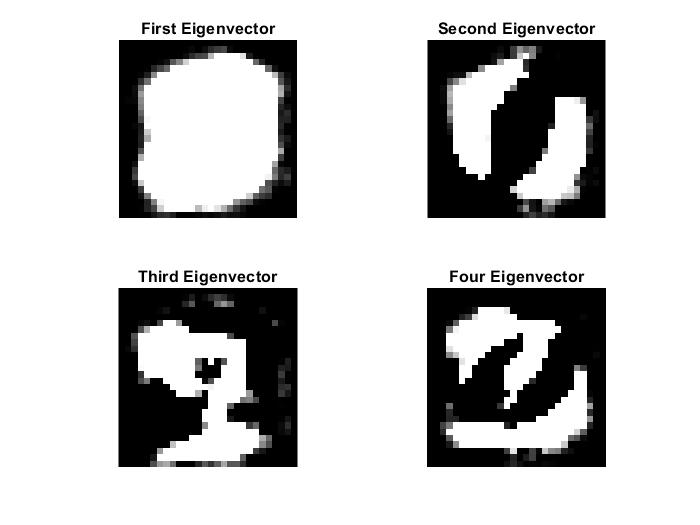
\includegraphics[width = 0.5\linewidth]{eigenvectors.jpg}
  \caption{Top 4 Eigenvector Visualization of Training Data Set Size: 600.}
\end{figure}

\noindent
It is important to note that the directionality of these vectors is wholy dependent on the input of our training data; meaning, our model will be incredibly susceptible to orientation differences amongst input images as well as additive noise.
\bigbreak
\noindent
In the following subsection, we will test the validity of our eigenvectors by visually inspecting how well we can reconstruct the image. 

\subsection{Test Digit Reconstruction}

Test digit reconstruction provides an excellent way to visually evaluate the effectiveness of our previously computed eigenvectors. Figure 2 (on the next page) shows the original  images from our testing set. Figure 3 shows the reconstruction of those digits. We can see in the reconstruction, artifacts from the transformation mapping which result in additional white pixels not found in the original images.

\begin{figure}[!htb]
    \centering
    \begin{tikzpicture}
    \node at (0,0) (a) {
\includegraphics[height=2cm]{7_orig.jpg}};
    \node[below = 2cm of a.south west,anchor= west] (b) {
\includegraphics[height=2cm]{2_orig.jpg}};
    \node[right = 1cm of a, anchor = west] (c) {
\includegraphics[height=2cm]{1_orig.jpg}};
    \node[below = 2cm of c.south east,anchor= east] (d) {
\includegraphics[height=2cm]{0_orig.jpg}};
    \end{tikzpicture}
    \caption{Original Test Images.}
\end{figure}

\begin{figure}[!htb]
    \centering
    \begin{tikzpicture}
    \node at (0,0) (a) {
\includegraphics[height=2cm]{7.jpg}};
    \node[below = 2cm of a.south west,anchor= west] (b) {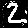
\includegraphics[height=2cm]{2.jpg}};
    \node[right = 1cm of a, anchor = west] (c) {
\includegraphics[height=2cm]{1.jpg}};
    \node[below = 2cm of c.south east,anchor= east] (d) {
\includegraphics[height=2cm]{0.jpg}};
    \end{tikzpicture}
    \caption{Reconstruction of Test Images.}
\end{figure}
\FloatBarrier

\noindent

Overall, despite the resulting discrepancies that stem from the generalized reconstruction method used in PCA, the resulting digits are recognizable to the human eye.

\subsection{The Size of Training Data and Its Impact on Accuracy}

The effects of training data size on the accuracy of the PCA model and KNN classification methods are discussed within this subsection. Figure 4 on the following page graphically illustrates the overall accuracy of my model with respect to the size of training data. 

\begin{figure}[!htb]
    \centering
    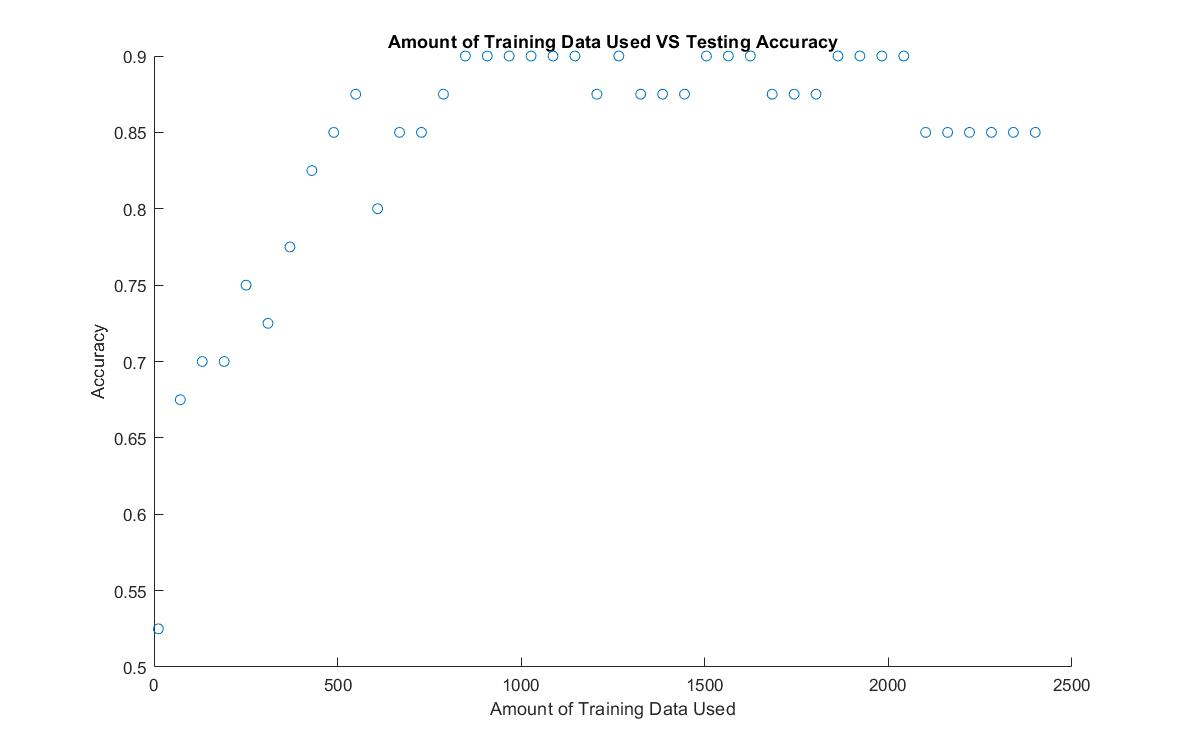
\includegraphics[width = 0.8\linewidth]{trainingdatavsaccuracy.jpg}
  \caption{The Effect of Training Data Size on Classification Accuracy}
\end{figure}
\FloatBarrier

\noindent
There is a clear trend in the graph above. As the amount of training data increases, the accuracy of the model increases up to a point (roughly 0.9 in this model.) In the graph above, an input size of 950 samples leads to a plateau in model accuracy. Thereafter, oscillation in accuracy in the model occurs until reaching 2000 input samples, at which point there begins to be a decline in accuracy. This decline could be the starting point of overfitting the large input data to the much smaller in size testing set data. 

\subsection{The Top N Eigenvectors’ Impact on Model Accuracy}

Principal Component Analysis (PCA) relies heavily on finding a coordinate system that best represents the variance in the data along various dimensions (number of dimensions relies on user choice.) Generally, we can determine the principal components or the dimensional axes of our model by finding the eigenvector and eigenvalues of the covariance matrix of our data. 

\bigbreak
\noindent
Once the eigenvectors and eigenvalues are known, the eigenvalues with the greatest weights correlate to the eigenvectors that span axes of the greatest variation. To explain furter, the first principal component of the model is represented by the eigenvector with the greatest associated eigenvalue and so forth. This information can be leveraged to empirically determine the best dimensional order of the subspace projection. 

\begin{figure}[!htb]
    \centering
    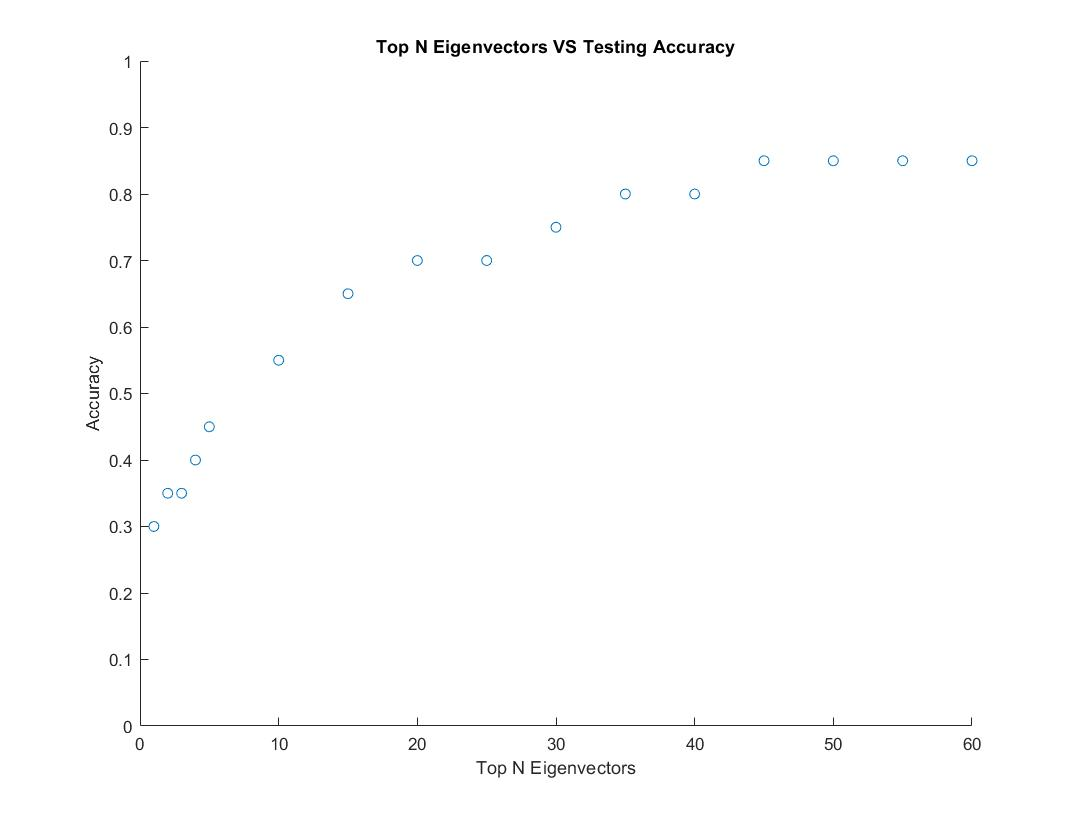
\includegraphics[width = 0.8\linewidth]{top_eigenvectors.jpg}
  \caption{Top N Eigenvectors Influence on Classification Accuracy}
\end{figure}
\FloatBarrier

\noindent
The figure above shows the overall effect of changing the dimensional order of the subspace based on the top N influential eigenvectors. Empirically we can determine that the curve flattens around the top 50 eigenvectors. Therefore it is possible to represent our training data at that reduced dimensional subspace with only little accuracy loss in the model.

\bigbreak
\noindent
There does exist an important caveat with this methodology. Thus far it has been assumed that the most discrimintive information is captured by the eigenvector with the greatest associated eigenvalue. However, there are cases where discriminitive information is contained in the directions of the smallest variance. Using PCA on classifications problems of this variety will negatively impact accuracy.

\subsection{Varying K and Its Impact on Model Accuracy }

After projecting the test image into the subspace used in the training step, a classification algorithm is performed to determine a label for the test image. The classification used in this report is a K Nearest Neighbors (KNN) search using euclidean distance to determine the nearest neighbor. Once the K nearest neighbors were chosen, the mode of the set of neighbors was chosen to label the test image.

\bigbreak
\noindent
The KNN algorithm is a non-parametric method that can be used for classification and regression problems. In the assignment given, KNN is used for classification. Once the test image is mapped to the subspace, the euclidean distance metric on the following page is used to determine the K nearest training examples closest to the test image.

\[D_{ij}^2 = \sum_{v=1}^{m} (x_{vi}-x_{vj})^2 \]

\noindent
\(D_{ij}\) represents the euclidean distance (note: you must take the square root of the equation above to achieve this.) The \(x\) variables represent differing points in N dimensional space. Once the K nearest points are calculated, the labels associated with those points are leveraged to determine the label of the test data. In my implementation, the statistical mode is used to determine the label of the test image.

\bigbreak
\noindent
The Figures 6 and 7 below depict how the change in K affects the the overall classification accuracy.

\begin{figure}[!htb]
    \centering
    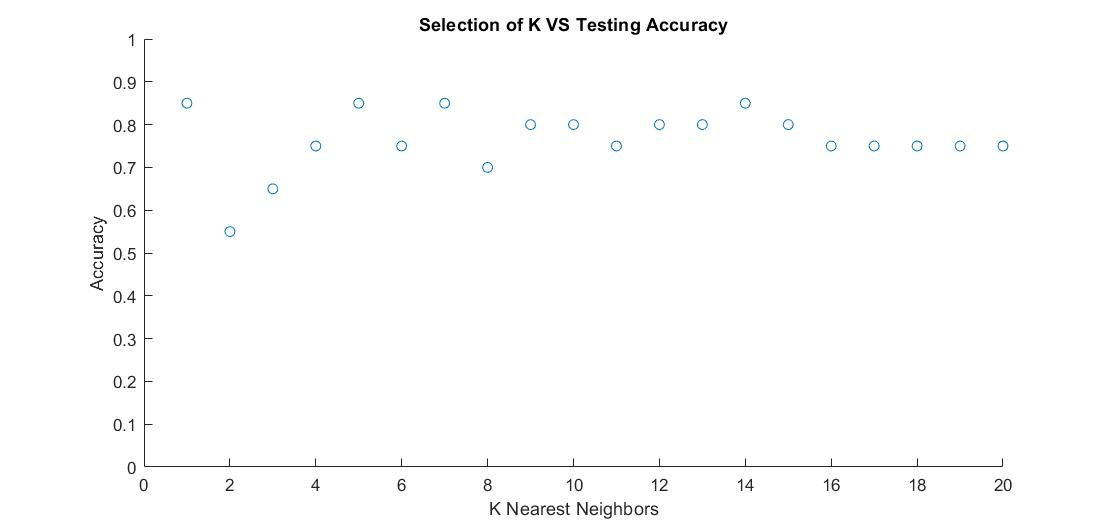
\includegraphics[width = 0.8\linewidth]{small_k.jpg}
  \caption{Selection of K between 1 and 20 in K Nearest Neighbor Algorithm and Its Effect on Classification Accuracy}
\end{figure}
\FloatBarrier

\noindent
In Figure 6, the accuracy of the model fluctuated until reaching K = 5. For K values greater than 5 and less than 20, the average model accuracy hovered around 0.80. 

\begin{figure}[!htb]
    \centering
    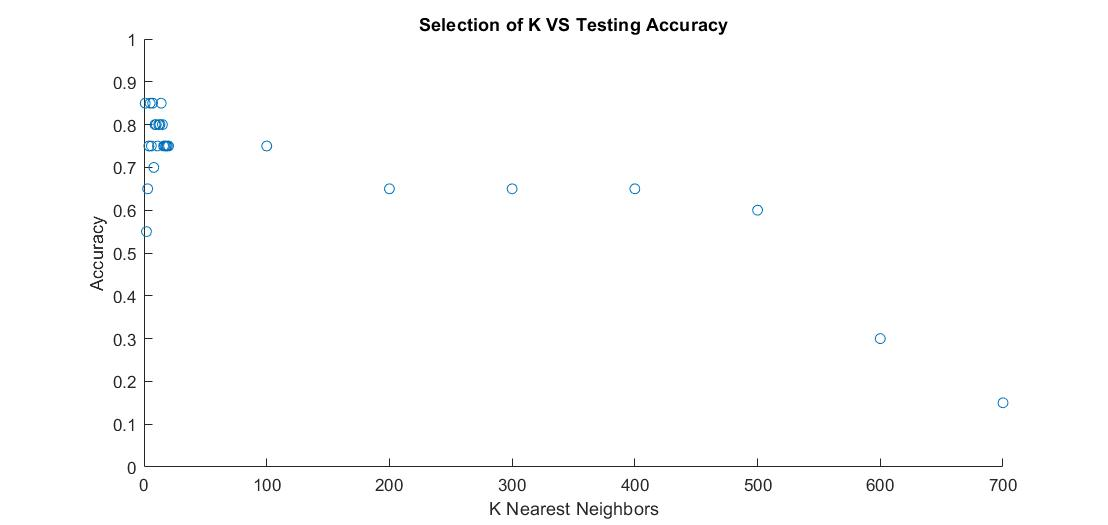
\includegraphics[width = 0.8\linewidth]{large_k.jpg}
  \caption{Selection of K between 1 and 700 in K Nearest Neighbor Algorithm and Its Effect on Classification Accuracy}
\end{figure}
\FloatBarrier

\noindent
Figure 7 above shows the impact of choosing very large K values relative to the total size of the training set. The training set data size chosen for this run was 729 input samples. A steady decline in accuracy is apparent from K values between 100 to 400. Around K=500, the model accuracy begins to plummet. This makes sense because as more garbage data is included in the large K clusters, the resulting modes are not representative of the data.

\bigbreak
\noindent
The optimal K values are as large as noise doesn't dominate and negatively effect the model accuracy and as small as a minority of data points don't dominate the accuracy either. Tuning this is difficult; however, as a rule of thumb, the square root of the total training data set is often used. Additionally, applying cross validation on a number of K values to empirically determine the best K is also a viable option. Through observation of figures 6 and 7, I chose K = 5 for the KNN classification used. A KNN of 5 maximized the overall probability of my models and provided robust results.

\section{Summary}

In this assignment, principal component analysis (PCA) was used for the purposes of feature extraction and mapping high dimensional data to low-dimensional data projections. Thereafter, a K Nearest Neighbors classification algorithm was used to label test images inputted to the PCA model. 

\bigbreak
\noindent
The overall accuracy of the produced model was roughly 0.90. Several additional steps could have been taken to further increase the accuracy of the model. First, additional training data could have supplemented the model by taking existing training data and rotating the images. Additionally, noise filtration examples could have been added to the model or the preprocessing steps before inputting test data into the model. 

\bigbreak
\noindent
The PCA method proved to be very effective in labeling handwritten digits from the MNIST data set. However, there are drawbacks to using PCA on image classification tasks. Primarily, by rearranging pixels in 1D column vector, relational information between the pixels is lost. Additionally, error in the input images influences the whole eigen-representation, this leads to a very big influence image noise has on the classification task.  

\end{document}
              